%課題研究レジュメテンプレート ver. 1.2

\documentclass[uplatex]{jsarticle}
\usepackage[top=20mm,bottom=20mm,left=20mm,right=20mm]{geometry}
\usepackage[T1]{fontenc}
\usepackage{txfonts}
\usepackage{wrapfig}
\usepackage[expert,deluxe]{otf}
\usepackage[dvipdfmx,hiresbb]{graphicx}
\usepackage[dvipdfmx]{hyperref}
\usepackage{pxjahyper}
\usepackage{secdot}


\makeatletter
  \renewcommand{\section}{%
    \if@slide\clearpage\fi
    \@startsection{section}{1}{\z@}%
    {\Cvs \@plus.5\Cdp \@minus.2\Cdp}% 前アキ
    {.5\Cvs \@plus.3\Cdp}% 後アキ
    %{\normalfont\Large\headfont\raggedright}}
    {\normalfont\raggedright}}

  \renewcommand{\subsection}{\@startsection{subsection}{2}{\z@}%
    {\Cvs \@plus.5\Cdp \@minus.2\Cdp}% 前アキ
    {.5\Cvs \@plus.3\Cdp}% 後アキ
    %{\normalfont\large\headfont}}
    {\normalfont}}

  \renewcommand{\subsubsection}{\@startsection{subsubsection}{3}{\z@}%
    {\Cvs \@plus.5\Cdp \@minus.2\Cdp}%
    {\z@}%
    %{\normalfont\normalsize\headfont}}
    {\normalfont}}
\makeatother
%ここから上を編集する必要はない.





\title{\vspace{-14mm}経常利益の予測と実数値}
\author{PMコース 矢吹研究室 1442020 大木崇雅}
\date{}%日付を入れる必要はない.
\pagestyle{empty}%ページ番号は振らない.
\begin{document}
\maketitle





\section{研究の背景}

1999年10月からインターネット上で株式のオンライントレードが可能になってから,株式がとても簡易に取引できるようになり株取引の普及が進んだ.株とは企業の資金調達のために発行している有価証券のことで,企業は株券を発行して集めた資金を使って事業を拡大する.株を買うことは,株を発行している企業に出資して事業資金を提供していることを意味する.株価は企業が今後大きな利益を上げると期待できる要因があると大きく上昇する.投資家は,今後の企業の成長性などに期待して株を買うが,投資する要因の1つとして挙げられるのが,経常利益である.なぜなら経常利益は売り上げからコストを差し引いた営業利益に財務活動などの損益を加えた数値であり,企業全体の強さが色濃く表れているからである.営業利益とは売上高からコスト(人件費や材料費,広告宣伝費)などを差し引いたもので本業で稼いだ利益のことである.従って経常利益は本業と副業を合わせた会社の実力を示す利益を意味する\cite{BA67886013}.例え小規模企業でも,経常利益4億円を実現できれば,東京証券取引所や大阪証券取引所の市場2部への上場の資格を得ることができるため,経常利益は株式市場への影響力が大きいと思われる.

企業の業績が下がれば株価も下がる場合が多いため,会社の実力である経常利益は株価への影響が大きい.株価と経常利益は大きく関係しあっているため,経常利益の予測ができれば株価も予測できると思われる.




\section{研究の目的}


本研究の目的は,四季報に掲載されている経常利益の予測値と実際の数値との差が少ない企業の業界を調べる事である.


\section{プロジェクトマネジメントとの関連}

本研究はリスクマネジメントに関連している.リーマンショック時やイギリスのEU離脱時など株式市場が混乱した際,株価と経常利益に大きく変動があるため,影響を受けた企業にどのようながリスクがあったのかというリスク特定に繋がると考えたからである.





\section{研究の方法}

東証一部に上場している約2000社の中から4分の1にあたる500社を調査し経常利益から得られる傾向を調べる.
予測の情報が記載されているサイトはスキャンで取り込んだ画像データを載せているサイトのため,画像データを視認してデータを打ち込んで取得する.経常利益の予測値を折れ線,実益値を棒グラフの複合グラフにして予測値と,実益値を可視化する.経常利益の予測値を実益値で割った結果が1に近いほど正確な予測ができているものとし,調査した年数分の平均値を求める.

\section{研究の結果}

500社中65社の26年分のデータを取得し,経常利益予測から実際の経常利益を割って出た値の大きさから65社を4種類に分類した.0.0001~0.00099までの値をAとし,0.001~0.0099までの値をBとし,0,01~0,099までの値をCとし,0.1~0.99までの値をDと分類した.値Aは2社,値Bは7社,値Cは27社,値Dは29社と分類された.予測との誤差の最も少ない値A,Bの9社中4社が運輸関連業であった.建設業と電気機器業が全体の24%を占め,化学業と陸運業が全体の21%を占めていた.電気機器メーカーの会社でも,商社も兼ね備えているという会社が多く,国外にも市場を展開しているという事がわかった.

以下の2社のモーターを作っている会社に,予測と実際の経常利益との差が少ない傾向にあった.さらにこれらの会社は株価の値動きと,経常利益の動き方が似た傾向を示している事が判明した.やはり共通点は国外にも市場を展開しているという事だった.以下の図は左が経常利益の予測値と実益値の推移で,右が株価の推移である.

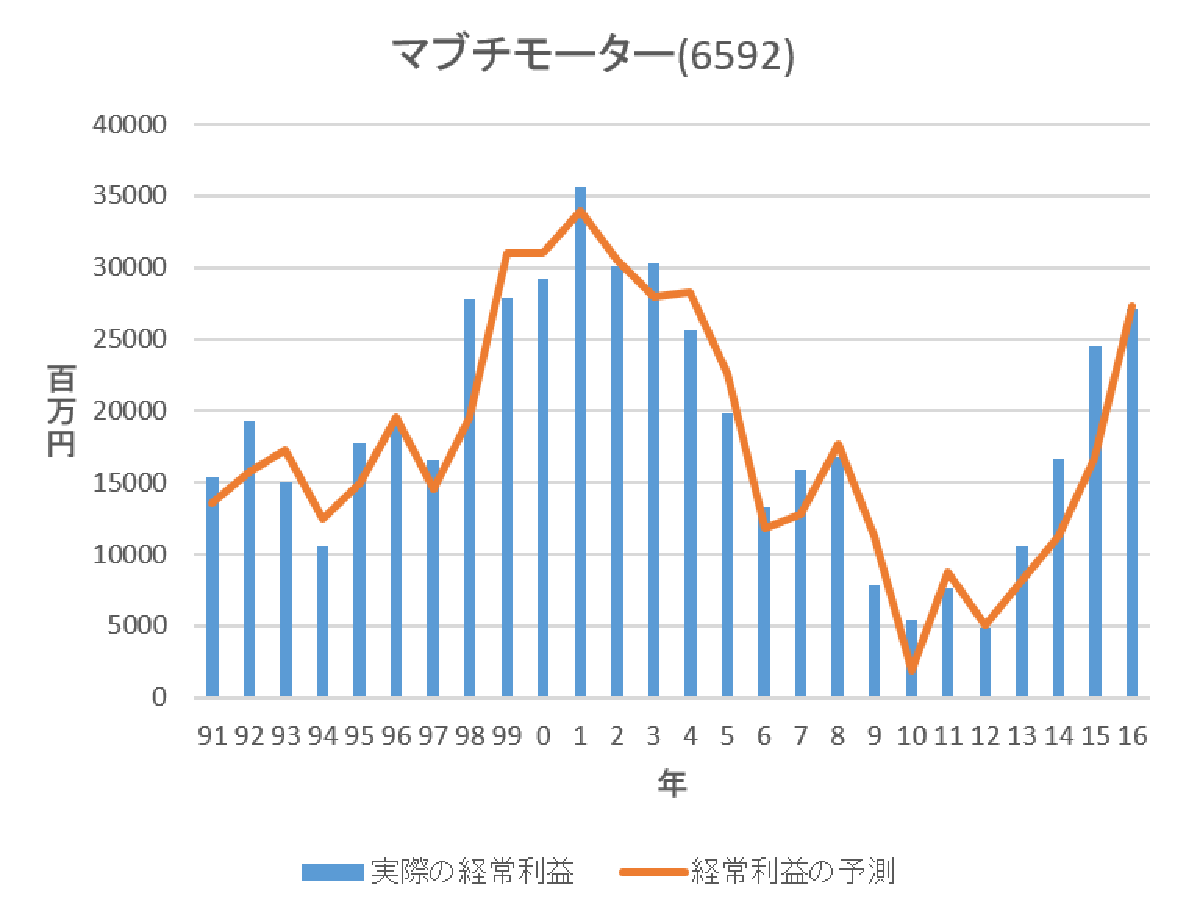
\includegraphics[width=8cm,height=7cm,bb=0 0 745 530]{mbtm.pdf}\cite{123} 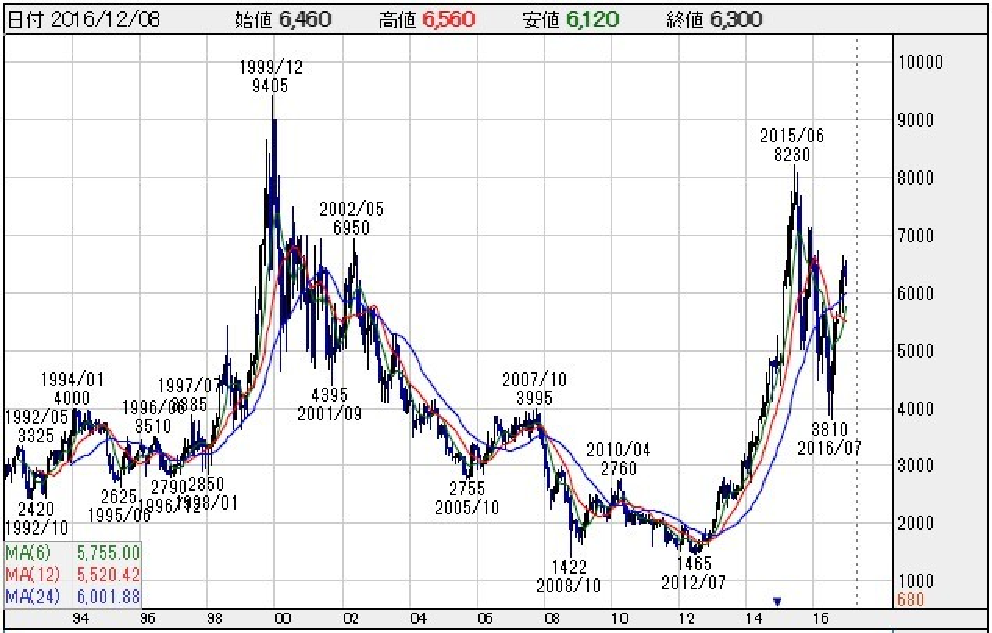
\includegraphics[width=8cm,height=7cm,bb=0 0 634 405]{mbtkbk.pdf}\cite{self}

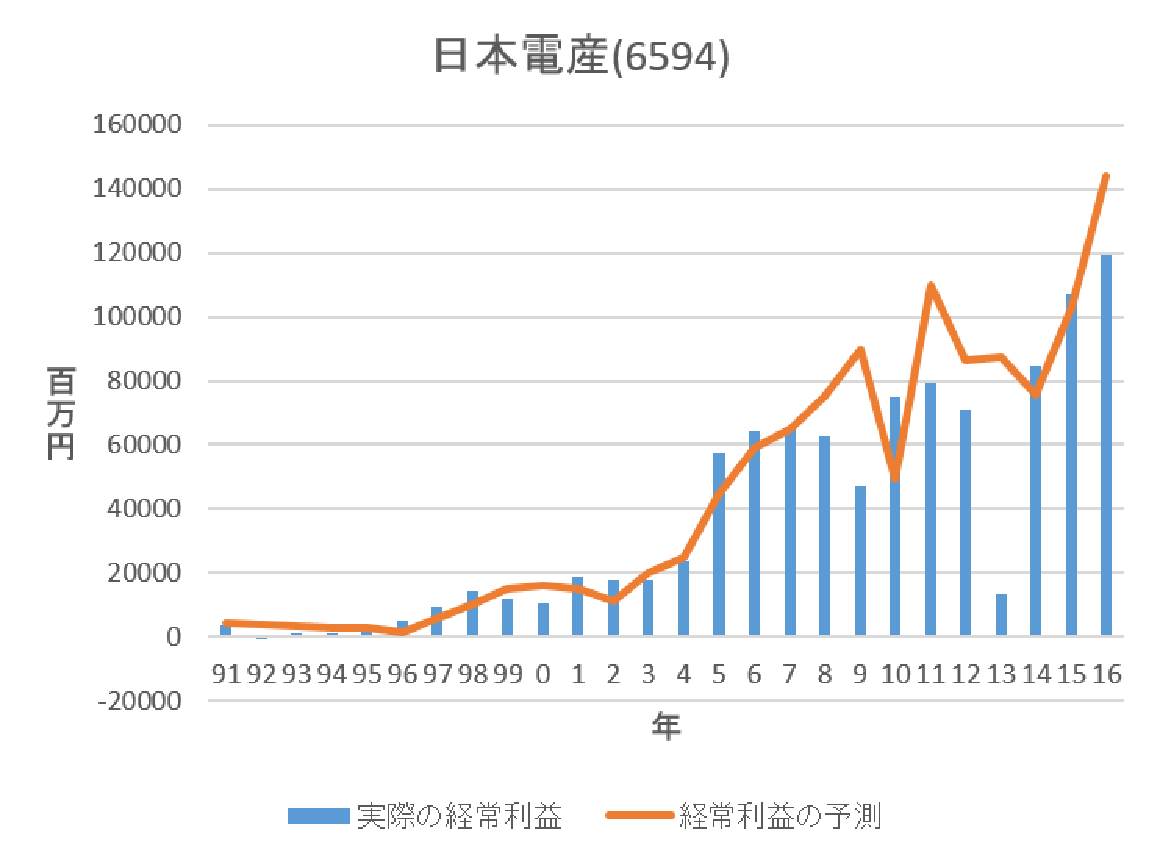
\includegraphics[width=8cm,height=7cm,bb=0 0 745 530]{densan.pdf}\cite{123} 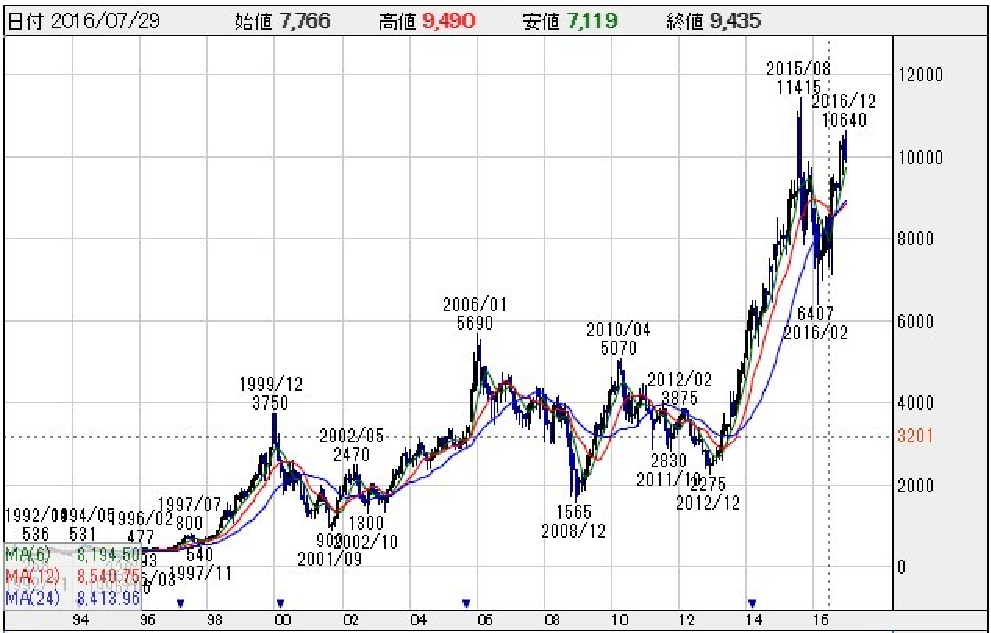
\includegraphics[width=8cm,height=7cm,bb=0 0 634 405]{densankbk.pdf}\cite{self}


\section{今後の計画}
現在取得した65社のサンプル数からより説得力のあるデータを作るため,今後も継続して経常利益の予測データを取得する.


\bibliographystyle{junsrt}
\bibliography{biblio}%「biblio.bib」というファイルが必要.

\end{document}